
\documentclass[lang=cn]{elegantpaper}
\setlength{\parskip}{1ex}
\linespread{1.5}
% title information
\title{网页画图软件系统报告} 
\author{靳学乾  刘学贵  李利娟  王汉镕  徐一舫}
%\version{1.00}%#\date{\today}
\usepackage{caption}
\usepackage{subfigure}
\usepackage{color}
\newcommand{\tabincell}[2]{\begin{tabular}{@{}#1@{}}#2\end{tabular}} 

\begin{document}

\begin{figure}
  \begin{minipage}{0.6\linewidth}
    
\includegraphics[width=0.6\linewidth]{logo.png}
  \end{minipage}
\end{figure}

\maketitle

\section{引言}

\subsection{项目背景}
为了将在软件工程课程所学理论知识转化成实践经验,增强对软件工程系统性的认识和了解,提升解决实际项目开发过程遇到问题的能力,我们小组合作完成网页作图这一项目。

通过本次综合设计,了解面向对象程序的开发思想、方法和步骤,掌握开发工具的使用,提高综合运用所学的理论知识和方法独立分析和解决问题的能力,进一步提高了设计实现网页的能力。

通过本次网页绘图软件的工程实践,我们掌握了前端开发语言的一些编程技巧,并学会了编写结构清晰、风格良好的、数据结构适当的程序,从而具备解决综合实际问题的能力。此外,我们还熟悉了网页设计创意的原理和方法,调动课内课外的主动性和积极性,促进对课程的全面掌握和理解。最后,我们练习使用了 HTML、CSS、JavaScript 这些前端编程语言, 熟悉了网页的制作流程,并且根据客户需求进行了网页设计与制作。总体而言,对于给定的软件需求,要学会如何进行分析,学会理清设计思路并给出相应的设计方案。

\subsection{编写目的}
书写本文档的目的在于:
\begin{itemize}
	\item [(1)]详细陈述网页作图软件工程需求,便于开发人员根据需求实现相应的功能;
	\item [(2)]明确软件设计思路和程序逻辑,便于维护人员进行后续维护工作;
	\item [(3)]展示测试过程以及现有效果,便于用户(此处指老师和同学)提出修改建议。
\end{itemize}

\subsection{读者对象和阅读建议}
本文档的主要内容分为三个部分:需求说明、系统说明、和测试部分。需求说明部分对网页作图系统的功能性需求和非功能性需求进行了详细描述,是开发人员进行开发时所参考的指导手册;系统说明部分描述了整个系统各个模块之间的关系,以及以主功能模块为例,对其中主要的程序接口进行说明;测试部分描述对系统进行测试的主要目的、方法、和过程。
本文档面向多类读者对象:
\begin{itemize}
	\item [(1)]开发人员:开发人员参考该文档尤其是需求说明部分,对系统各模块进行开发、维护。
	\item [(2)]测试人员:根据本文档的需求说明,对该系统进行功能性和非功能性测试。
	\item [(3)]用户:可以借助本文档了解网页作图系统具有的功能,了解使用系统功能,提出使用反馈意见。
\end{itemize}

\section{可行性分析}
我们主要从网页作图项目涉及到的基础知识以及目前网上类似工具调研两方面对这个项目的可行性进行分析,从而决定完成老师布置的关于网页作图题目,而不是换成其他项目。
\subsection{基础知识调研}
\subsubsection{HTML}
HTML的英文全称是 Hyper Text Markup Language,即超文本标记语言。使用HTML,将所需要表达的信息按某种规则写成HTML文件,通过专用的浏览器来识别,并将这些HTML文件“翻译”成可以识别的信息,即现在所见到的网页。自1990年以来,HTML就一直被用作WWW的信息表示语言,使用HTML描述的文件需要通过WWW浏览器显示出效果。

HTML是一种建立网页文件的语言,通过标记式的指令(Tag),将影像、声音、图片、文字动画、影视等内容显示出来。HTML的普遍应用就是带来了超文本的技术―通过单击鼠标从一个主题跳转到另一个主题,从一个页面跳转到另一个页面,与世界各地主机的文件链接超文本传输协议规定了浏览器在运行HTML文档时所遵循的规则和进行的操作。HTTP的制定使浏览器在运行超文本时有了统一的规则和标准。

\subsubsection{CSS}
CSS,层叠样式表(英文全称:Cascading Style Sheets)是一种用来表现HTML(标准通用标记语言的一个应用)或XML(标准通用标记语言的一个子集)等文件样式的计算机语言。CSS不仅可以静态地修饰网页,还可以配合各种脚本语言动态地对网页各元素进行格式化。 CSS 能够对网页中元素位置的排版进行像素级精确控制,支持几乎所有的字体字号样式,拥有对网页对象和模型样式编辑的能力。

\subsubsection{JavaScript}
JavaScript(简称“JS”) 是一种具有函数优先的轻量级,解释型或即时编译型的编程语言。虽然它是作为开发Web页面的脚本语言而出名,但是它也被用到了很多非浏览器环境中,JavaScript 基于原型编程、多范式的动态脚本语言,并且支持面向对象、命令式和声明式(如函数式编程)风格。

JavaScript是一种属于网络的高级脚本语言,已经被广泛用于Web应用开发,常用来为网页添加各式各样的动态功能,为用户提供更流畅美观的浏览效果。通常JavaScript脚本是通过嵌入在HTML中来实现自身的功能的。是一种解释性脚本语言(代码不进行预编译)。主要用来向HTML(标准通用标记语言下的一个应用)页面添加交互行为。 可以直接嵌入HTML页面,但写成单独的js文件有利于结构和行为的分离。\\


简单来说,上面三种分别实现这些功能:html负责内容,css负责样式,js负责控制。


\subsection{类似工具调研}

我们平时作图一般使用word或者visco这样的软件,这类软件虽然功能齐全,但有时候不是很方便,安装繁琐。因此如果可以实现网页作图的话,对于满足我们日常作图需求还是很有意义的。

现在网上已经有类似的作图网页,但是能够达到课程要求并且可以根据需求随时修改内容的作图网页还是没有,要么是功能过于简单,要么就是操作起来有些复杂。\\


总之,通过了解相关知识和对于网页作图难易程度的调研、需要的开发环境具备情况以及老师课上的分析讲解,我们认为网页绘图系统的开发是可行的,但实现起来并不简单,尤其是在我们小组成员都没有网页开发经验的情况下。通过一学期的学习和尝试,我们小组基本实现了系统的预期功能。网页绘图系统的实现对于小组成员快速学习知识并且通过新知进行一定程度的产出能力起到了非常好的锻炼效果。

\section{需求说明}
\subsection{功能性需求说明}

\subsubsection{根据函数绘制图形}
\begin{itemize}
	\item [(1)]自由输入函数,设置函数图形样式,绘制出对应的函数图形,在图例上标注函数名称和对应样式;
	\item [(2)]增加、删除需绘制的函数;
	\item [(3)]鼠标拖动、缩放绘制出的函数图形,并同步修改坐标轴范围;
	\item [(4)]能将移动后的函数图形恢复至原位;
	\item [(5)]设置图像标题、坐标轴名称以及坐标轴的取值范围。
\end{itemize}

\subsubsection{控制鼠标自由绘图}
\begin{itemize}
	\item [(1)]画笔:控制鼠标自由绘制图形;
	\item [(2)]设置线的颜色和粗细。
	\item [(3)]橡皮擦:擦除已绘制图形;
	\item [(4)]清屏:将画布自由绘制的图形全部擦除;
\end{itemize}

\subsubsection{插入规则图形}
\begin{itemize}
	\item [(1)]插入直线、向量、圆、矩形等规则图形,并能控制插入图形样式;
	\item [(2)]修改已插入图形的位置;
	\item [(3)]对直线、向量进行任意角度旋转、拉伸;
	\item [(4)]对圆、矩形进行大小缩放;
	\item [(5)]鼠标左击选中规则图形按Delete键进行删除操作。
\end{itemize}
	
\subsubsection{插入文字}
\begin{itemize}
	\item [(1)]输入文字在画布上显示;
	\item [(2)]设置字体颜色、大小;
	\item [(3)]移动文字改变其显示位置;
	\item [(4)]鼠标左击选中文字按Delete键进行删除操作。
\end{itemize}

\subsection{非功能性需求说明}
\subsubsection{网页界面}
具有优秀的功能设计和UI设计,符合多数用户的使用习惯,操作简单明了没有歧义,容错性好。

\subsubsection{鲁棒性}
确保网页不会因为操作系统、浏览器的变化出现访问不正常现象。

\section{开发计划}
我们小组在学期初经过一次讨论后,将网页绘图工程实践分为以下五个阶段:


阶段一:理解和整理各项需求,写好需求文档。确定好将网页端分为多少个功能模块,各功能模块又包含多少子功能模块,并确认好各功能模块之间是否存在联系以及存在什么样的联系,定下网页端的设计方向;并且根据模块划分将开发任务分配到具体的开发人员。

阶段二:根据阶段一确定下的设计方向,进行原型的设计开发,大致完成页面的总体设计。

阶段三:完成各个功能模块,并且将这些模块优化整合,实现我们预先定好的设计目标。

阶段四:测试人员考虑用户可能存在的各种需求,在此基础上设计测试方案,对网页进行各项测试,给出反馈,开发人员根据反馈进行相应的改善。

阶段五:撰写系统文档,详细描述作图网页的开发过程,总结这次实践经历和小组成员心得体会。


\section{系统说明}
\subsection{系统模块说明}


如图\ref{1img}所示,网页绘图系统功能分为主功能-函数绘制和辅助功能两大模块,其中,辅助功能又由涂鸦板、图形插入、文字插入三个部分组成。
\begin{figure}[htbp]
	\centering
	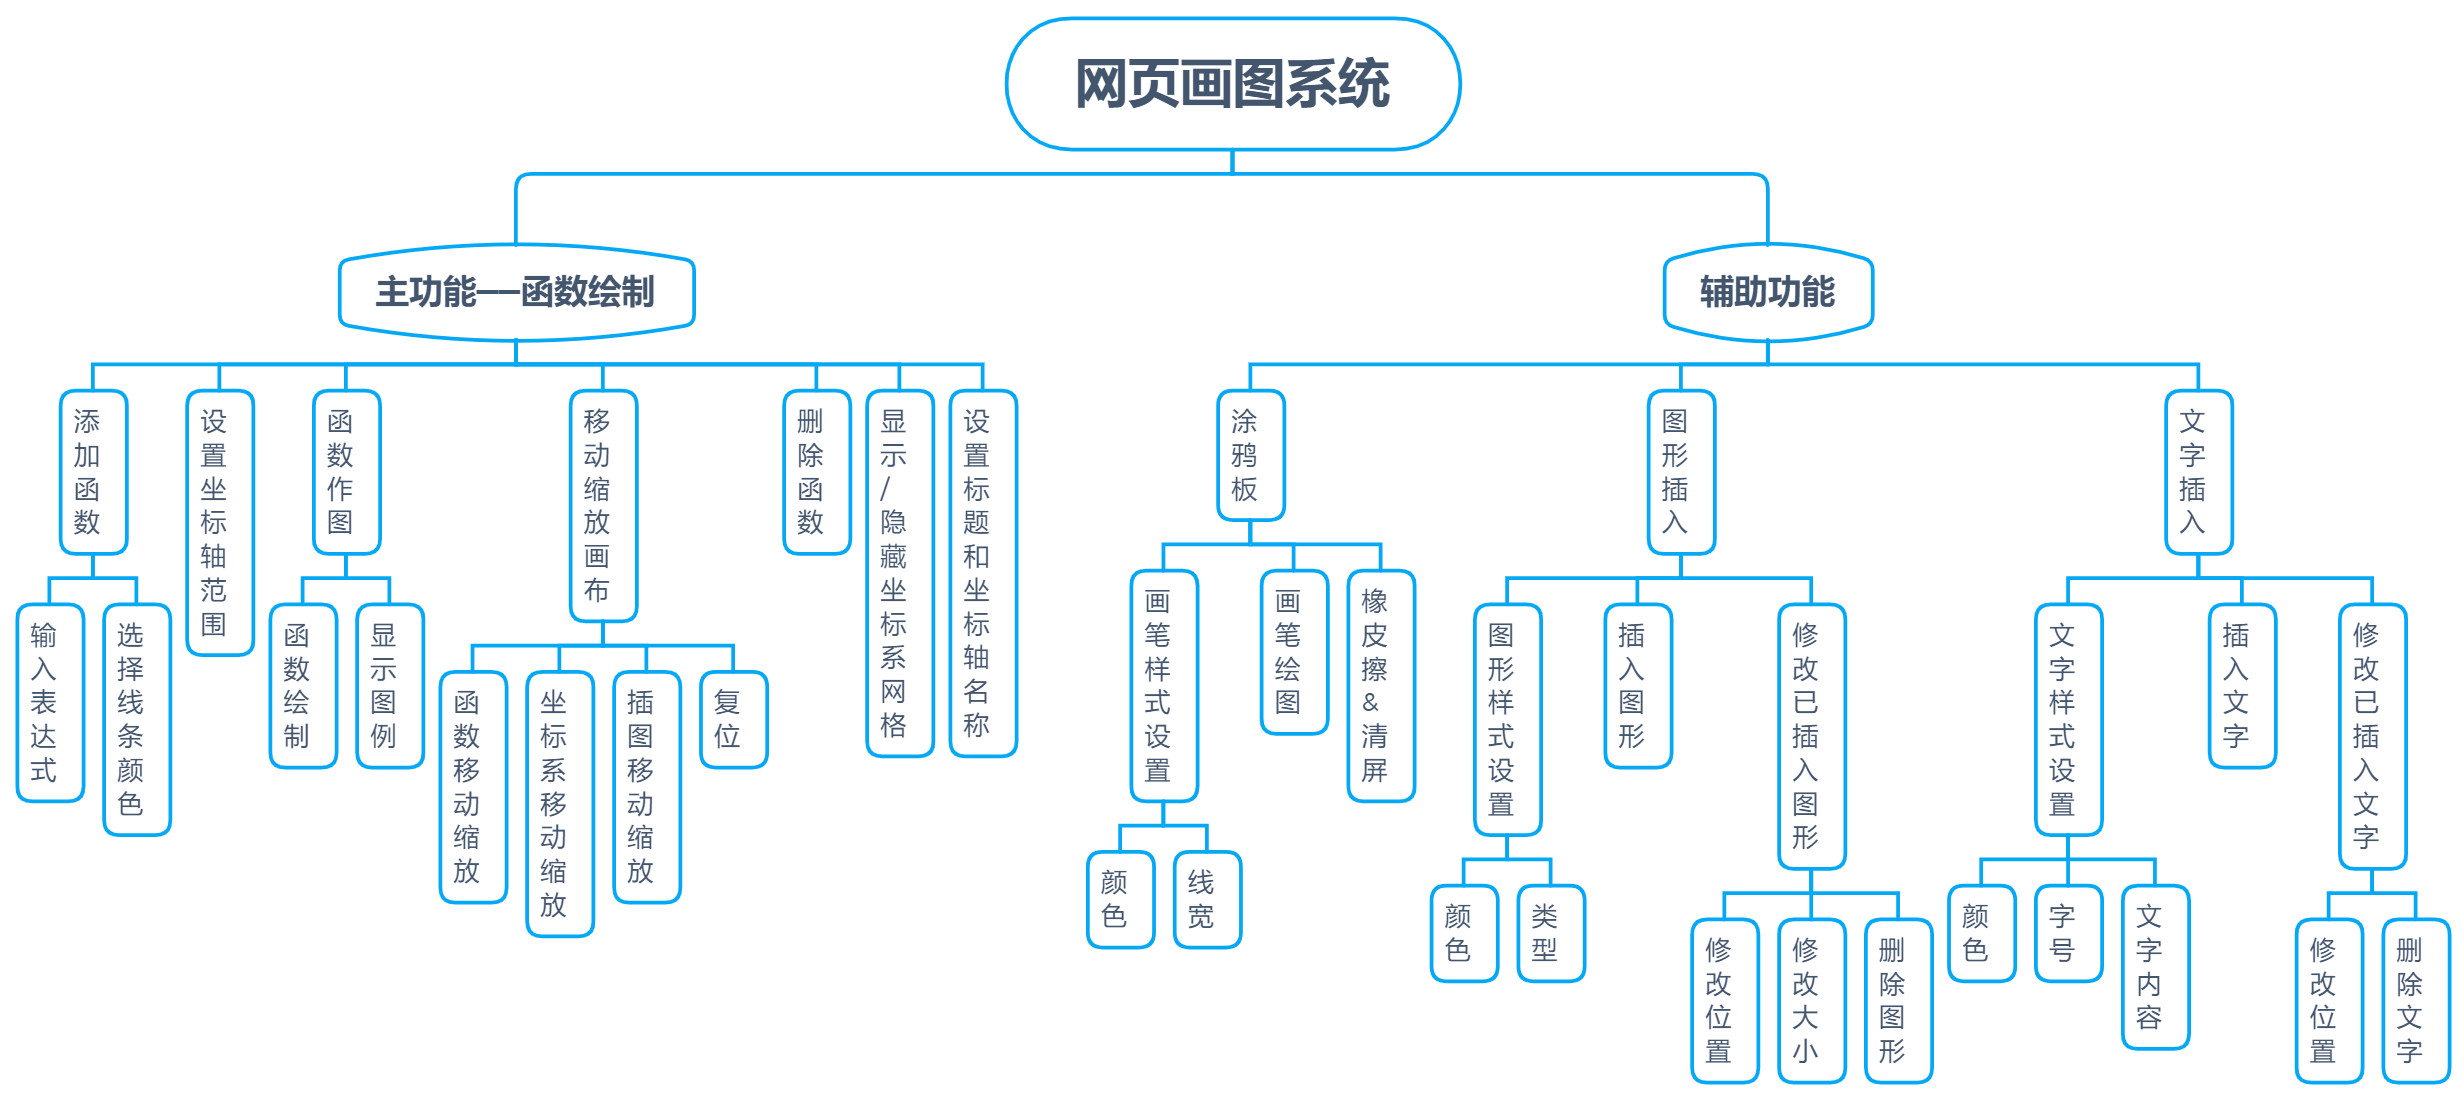
\includegraphics[width=1.0\textwidth]{1.png}
	\caption{网页绘图系统模块示意图}
	\label{1img}
\end{figure}

\subsection{设计思路}
\begin{itemize}
	\item [(1)]建立主功能模块各类事件程序接口,监听用户操作,实现相应的功能需求;
	\item [(2)]建立辅助功能模块事件程序接口;
	\item [(3)]参考状态机,添加事件相关函数和各监听事件,在主功能模块中监听辅助功能模块事件发生,进而调用相关函数,实现主功能和辅助功能的切换。
\end{itemize}

\subsection{程序接口描述}

以下为各模块部分函数接口的描述,更多程序接口描述见代码注释
\subsubsection{函数绘图}
\begin{center}
   	\fcolorbox{black}{gray!10}{\parbox{.9\linewidth}{calculate(fun, X, Value) 根据函数表达式和给定x取值计算函数y值
   			
   			value2PointY(y) 将 y 的计算数值转化为画布上的 y 像素位置
   			
   			drawLine(lx, ly, px, py) 根据x值和y值绘制曲线
   			
   			addFun() 增加函数
   			
   			deleteFun(node) 删除函数
   			
   			resetFun() 将图像复位
   			
   			addLegend(color, text) 增加标注
   			
   			delLegend() 删除标注
   			
   			updateLegend() 更新标注}}
\end{center}

\subsubsection{涂鸦板绘图}
\begin{center}
	\fcolorbox{black}{gray!10}{\parbox{.9\linewidth}{
			
			freestylePencil()  打开涂鸦板辅助功能
			
			fsCanvas.addEventListener('mousedown', fsPencilMouseDown = function (e) 添加画笔事件
			
			freestylePencil() 打开橡皮擦功能
			
			clearArea() 清屏}}
\end{center}

\subsubsection{插入图形}
\begin{center}
	\fcolorbox{black}{gray!10}{\parbox{.9\linewidth}{addGeom() 添加规则图形
			
			redrawGeom() 根据像素坐标绘制图形
			
			movingGeom() 移动插入的规则图形
			
			changeGeom() 修改插入的规则图形}}
\end{center}

\subsubsection{插入文字}
\begin{center}
	\fcolorbox{black}{gray!10}{\parbox{.9\linewidth}{addText() 添加文字
			
			redrawText() 根据像素绘制文字
			
			movingText() 移动文字
			
			changeText() 修改文字
			
			hitText(x1, y1, x2, y2, x, y) 选中文字}}
\end{center}

\section{测试}
\subsection{合法性检查}
检查开发人员在编写课程项目代码时使用的开发工具是否合法。对在编程中使用的不是由开发工具提供的控件、组件、函数库等,检查其是否有合法的发布许可。

\subsection{软件代码测试}
\subsubsection{源代码一般性检查}


\makeatletter\def\@captype{table}\makeatother

%\begin{table}  
   	\small
   	\caption{命名规范检查}  
   	\begin{center}  
   	\setlength{\tabcolsep}{7mm}{
	   	\resizebox{\textwidth}{!}{
   		\begin{tabular}{|l|l|l|l| |}  
   			\hline  
   			\tabincell{l}{测试目标 }& \tabincell{c}{检查源代码中的变量、函数、对象、过程等的命名是否符合约定规范,\\该规范由开发人员在写代码前商量约定,并且写入工程文档中 }\\ \hline  
   			测试方法和技术 & 根据软件工程文档的约定,对代码进行检查 \\ \hline  
   			完成标准 & 系统中重要部分都按规定命名\\  
   			\hline  
   		\end{tabular}  }}
   	\end{center}  
%\end{table}

%begin{table}  
	\small  
	\caption{注释检查}  
	\begin{center}  
	\setlength{\tabcolsep}{7mm}{
		\resizebox{\textwidth}{!}{
		\begin{tabular}{|l|l|l|l| |}  
			\hline  
			测试目标 & 检查程序中的注释是否规范,注释量是否达到约定要求\\ \hline  
			测试方法和技术 & 让测试人员对代码进行检查 \\ \hline  
			完成标准 & 测试人员能根据代码读懂代码并运行,可以进行后面其他测试\\  
			\hline  
		\end{tabular}  }}
	\end{center}  
%\end{table}

\subsubsection{软件一致性检查}
\begin{itemize}
	\item [(1)]编译检查:
	要求提交的源代码在其规定的编译环境中,能够重新编译无错误,并且能够完成相应的功能,从而确定上交给老师的代码是正确的源代码。
	\item [(2)]移植检查:
	要求提交的源代码移植到新的系统环境中也能顺利编译运行,实现要求的功能。
\end{itemize}


\subsection{软件功能测试}

\subsubsection{测试函数绘图}

\makeatletter\def\@captype{table}\makeatother	
%\begin{table}  
	\small
	\caption{测试函数绘图}  
	\begin{center}  
		\resizebox{\textwidth}{!}{
		\begin{tabular}{|l|l|l|l| p{8cm}|}  
			\hline  
			测试目标 & 输入不同的函数表达式,能否正确绘制出相应的图像,测试添加、删除函数是否方便快捷,能否移动缩放图像\\ \hline  
			测试方法和技术 & 让测试人员输入不同类型的函数 \\ \hline  
			完成标准 & 输入不同类型函数都可以输出正确图像,能方便添加删除函数,能移动缩放图像\\  
			\hline  
		\end{tabular}}  
	\end{center}  
%\end{table}

\begin{figure}[htbp]
	\centering
	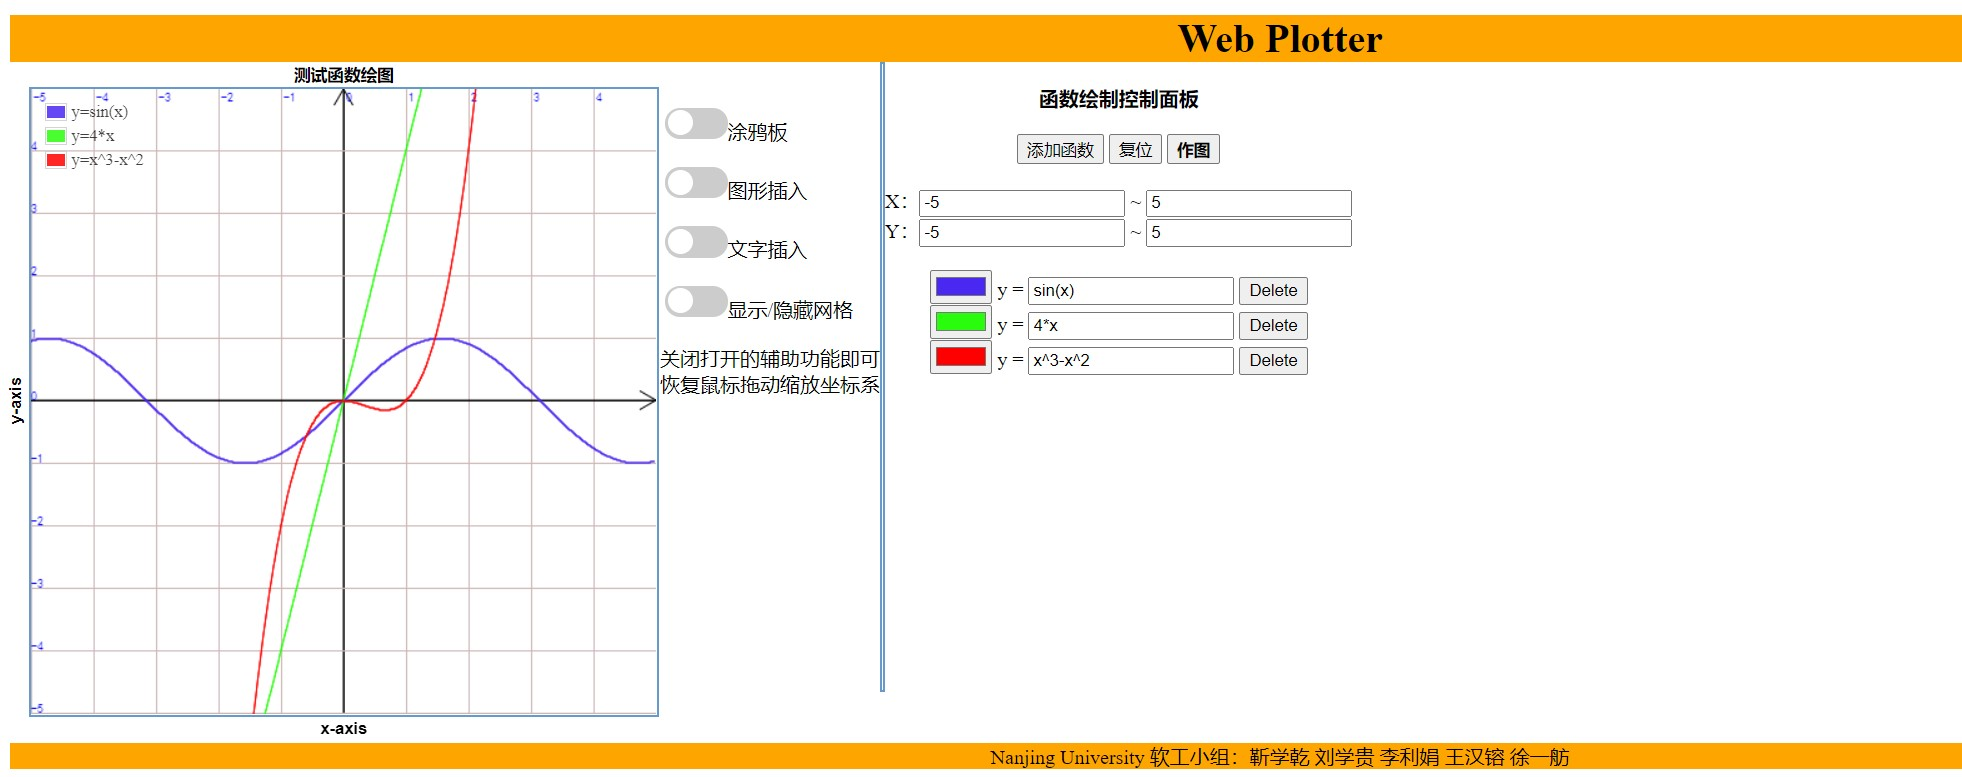
\includegraphics[width=1.0\textwidth]{2.jpg}
	\caption{根据函数表达式绘图效果}
	\label{2img}
\end{figure}

\begin{figure}[htbp]
	\centering
	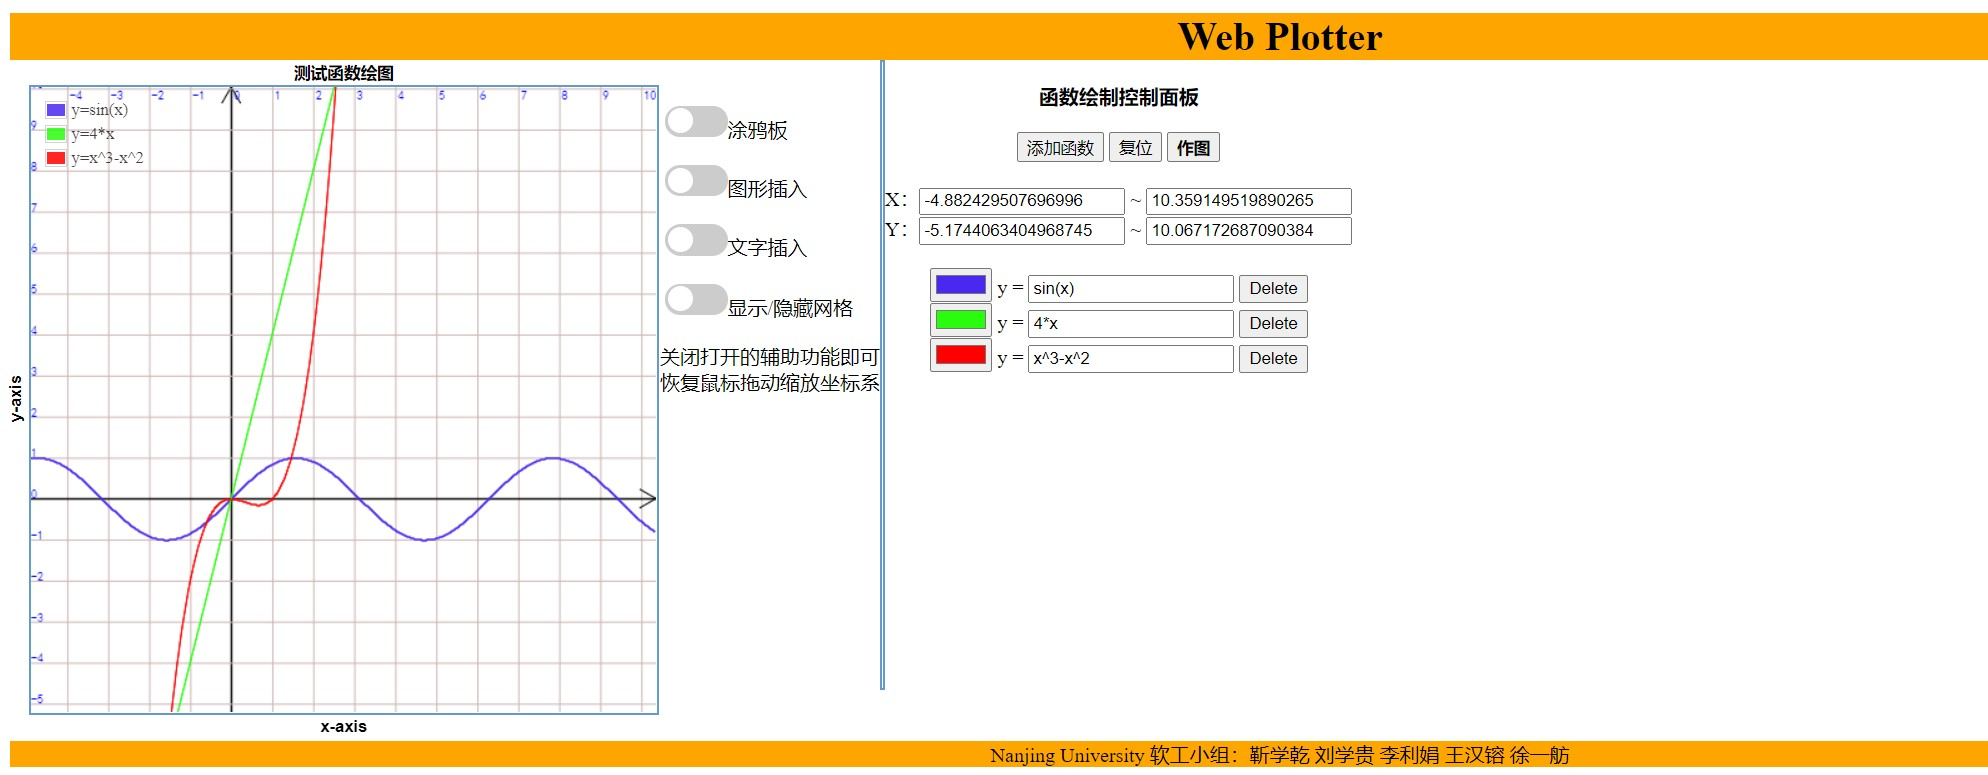
\includegraphics[width=1.0\textwidth]{3.jpg}
	\caption{移动缩放画布效果}
	\label{3img}
\end{figure}



\subsubsection{测试涂鸦板}
\makeatletter\def\@captype{table}\makeatother
%\begin{table}  
	\small
	\caption{测试涂鸦板}  
	\begin{center}  
		\resizebox{\textwidth}{!}{
		\begin{tabular}{|l|l|l|l| p{8cm}|}  
			\hline  
			测试目标 & 可以通过控制鼠标在网页自由绘图,并且能够擦除已绘制的图像\\ \hline  
			测试方法和技术 & 让测试人员移动鼠标在画布上自由绘图 \\ \hline  
			完成标准 & 画笔能及时准确响应鼠标的控制,橡皮擦能够实现对画布任意位置的擦除功能\\  
			\hline  
		\end{tabular}  }
	\end{center}  
%\end{table}

\begin{figure}[htbp]
	\centering
	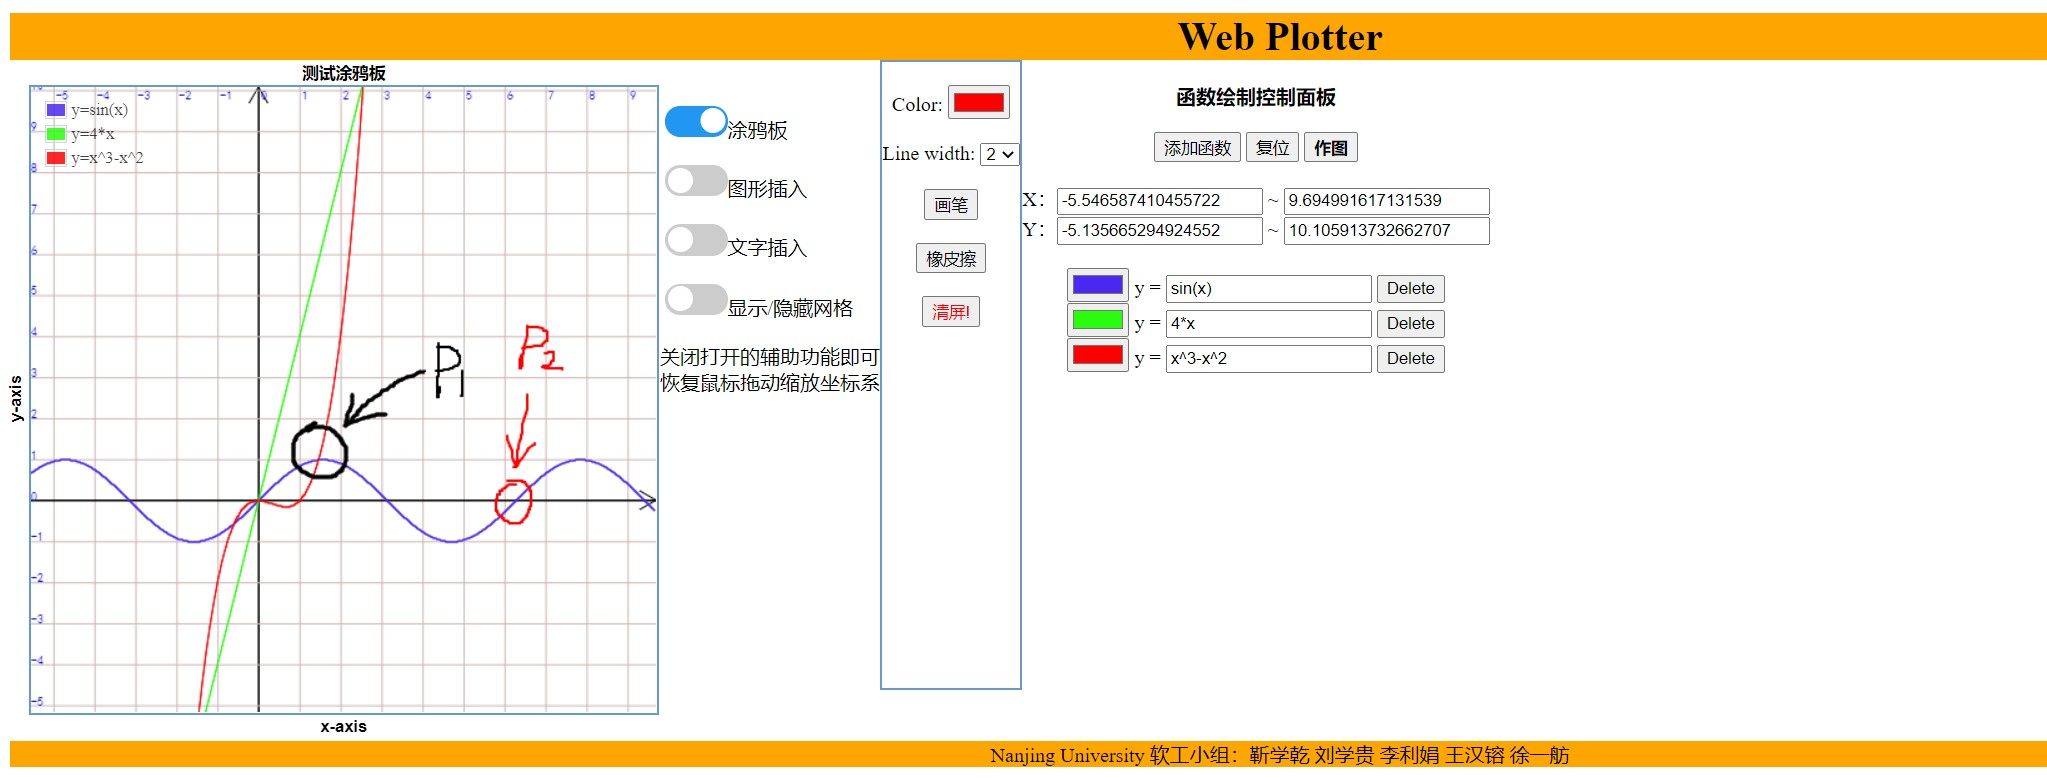
\includegraphics[width=1.0\textwidth]{4.jpg}
	\caption{测试涂鸦板画图效果}
	\label{4img}
\end{figure}



\subsubsection{测试图形插入功能}
\makeatletter\def\@captype{table}\makeatother
%\begin{table}  
	\small
	\caption{测试图形插入}  
	\begin{center}  
		\resizebox{\textwidth}{!}{
		\begin{tabular}{|l|l|l|l| p{8cm}|}  
			\hline  
			测试目标 & 可以插入圆、矩形、直线等规则图形和向量,能修改其位置和大小,并能拖动缩放\\ \hline  
			测试方法和技术 & 让测试人员选择插入不同颜色、不同形状的图形 \\ \hline  
			完成标准 & 图形正确插入到对应的位置,并且能修改其大小位置、拖动缩放\\  
			\hline  
		\end{tabular}  }
	\end{center}  
%\end{table}

\begin{figure}[htbp]
	\centering
	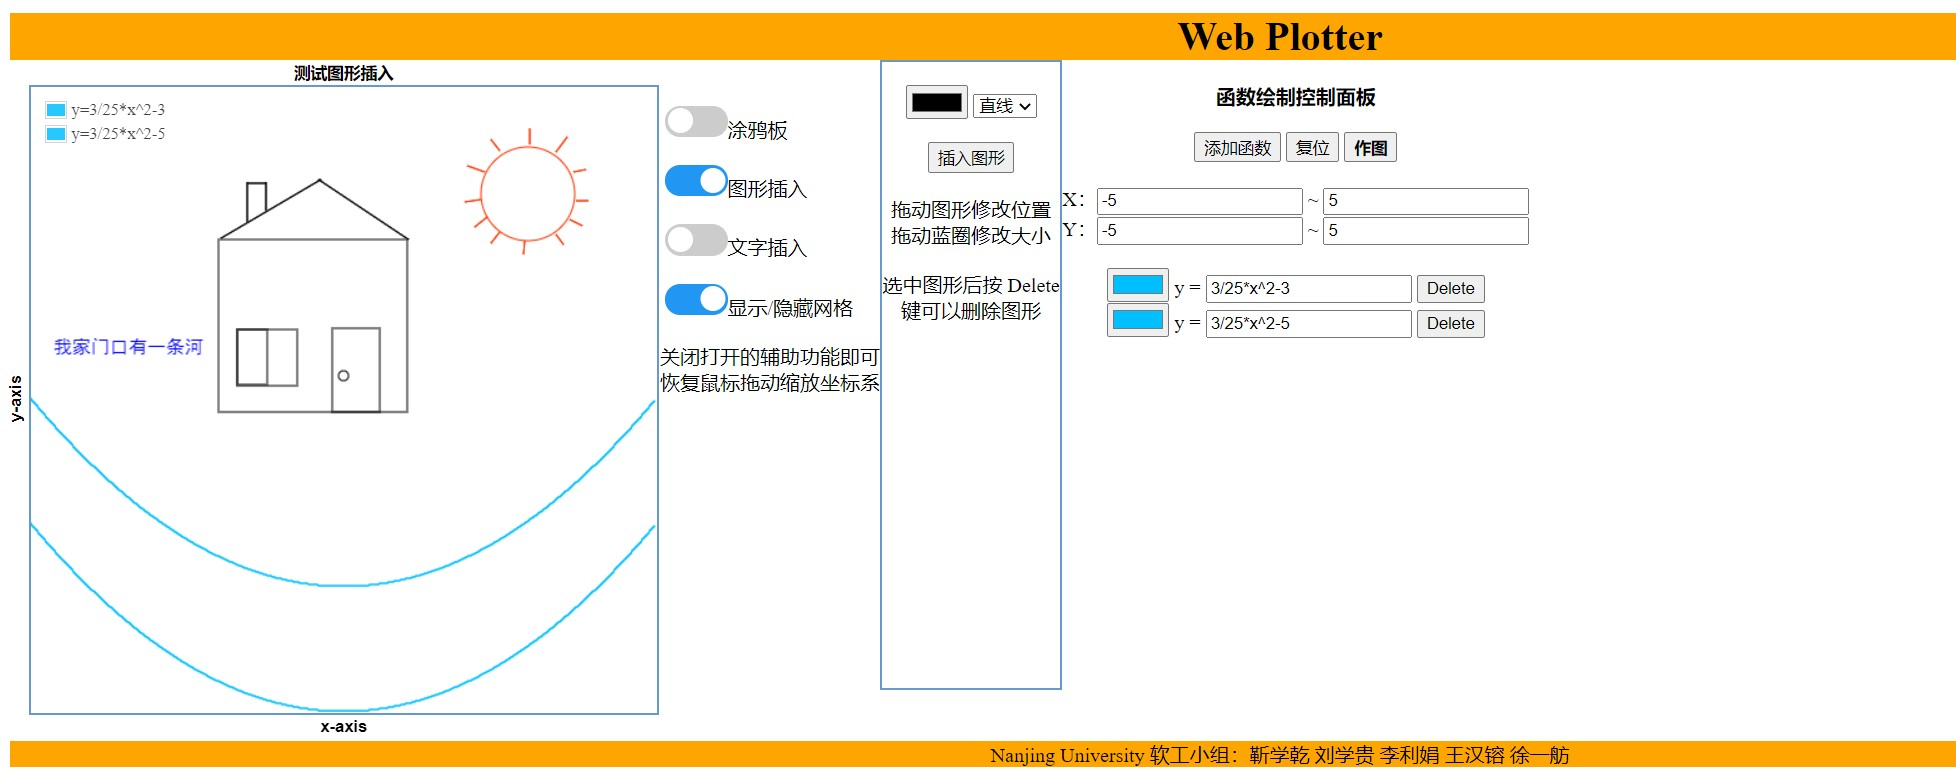
\includegraphics[width=1.0\textwidth]{6.jpg}
	\caption{测试图形插入效果}
	\label{6img}
\end{figure}

\begin{figure}[htbp]
	\centering
	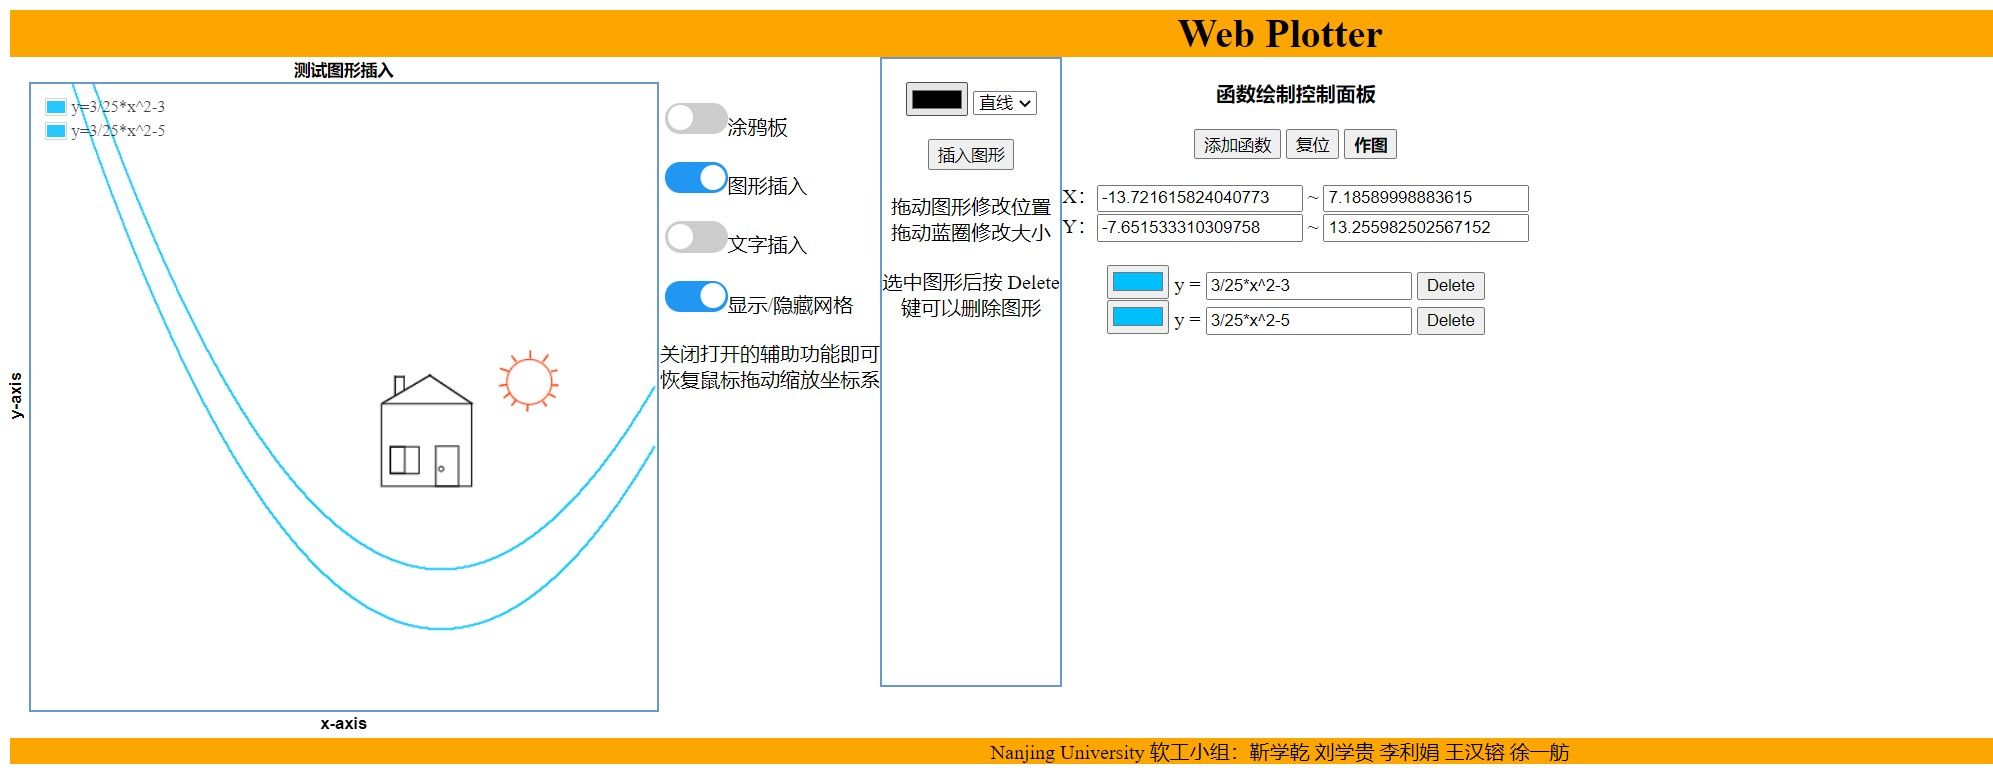
\includegraphics[width=1.0\textwidth]{7.jpg}
	\caption{测试图形拖动缩放效果}
	\label{7img}
\end{figure}

\begin{figure}[htbp]
	\centering
	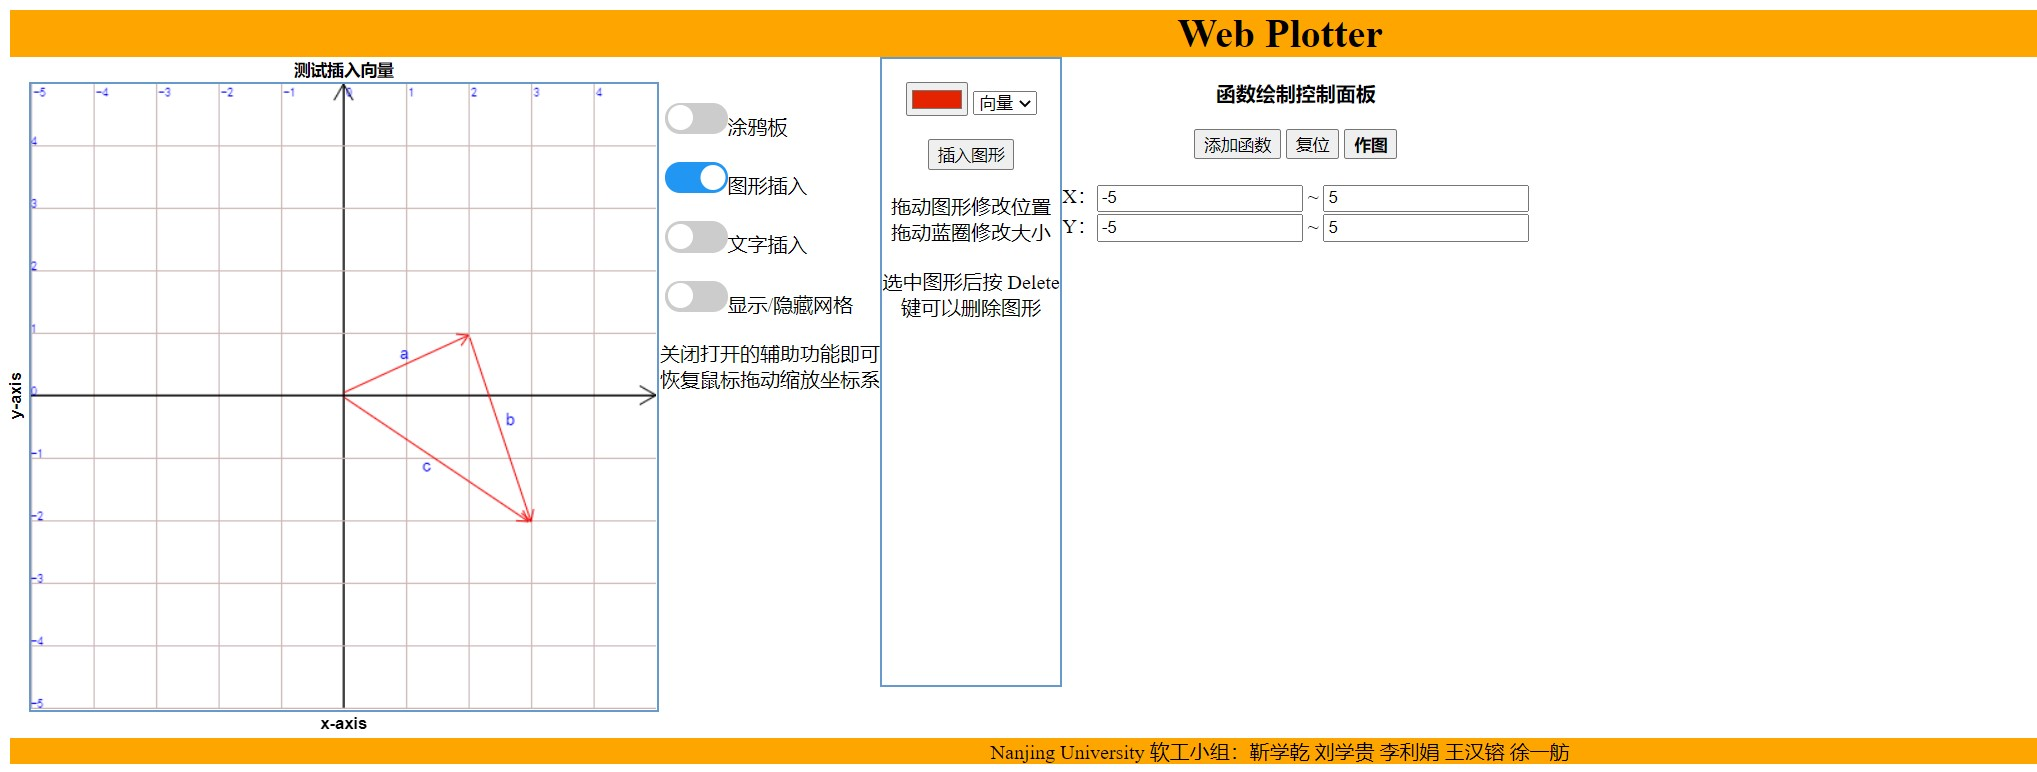
\includegraphics[width=1.0\textwidth]{8.jpg}
	\caption{测试插入向量效果}
	\label{8img}
\end{figure}

图\ref{6img}展示了由函数、图形共同构成的一副画作,用到了不同的图形;图\ref{7img}展示了鼠标拖动缩放整幅图像后的效果,可以看到,函数和图形均显示在了正确位置;图\ref{8img}展示了插入向量功能的效果图。

\subsubsection{测试文字插入功能}

\makeatletter\def\@captype{table}\makeatother
%\begin{table}  
	\small
	\caption{测试文字插入}  
	\begin{center}  
		\resizebox{\textwidth}{!}{
		\begin{tabular}{|l|l|l|l| p{8cm}|}  
			\hline  
			测试目标 & 可以插入不同大小、颜色的文字,能够改变文字出现位置、删除文字\\ \hline  
			测试方法和技术 & 让测试人员选择插入不同大小、颜色的文字 \\ \hline  
			完成标准 & 文字能正常显示\\  
			\hline  
		\end{tabular}  }
	\end{center}  
%\end{table}

\begin{figure}[htbp]
	\centering
	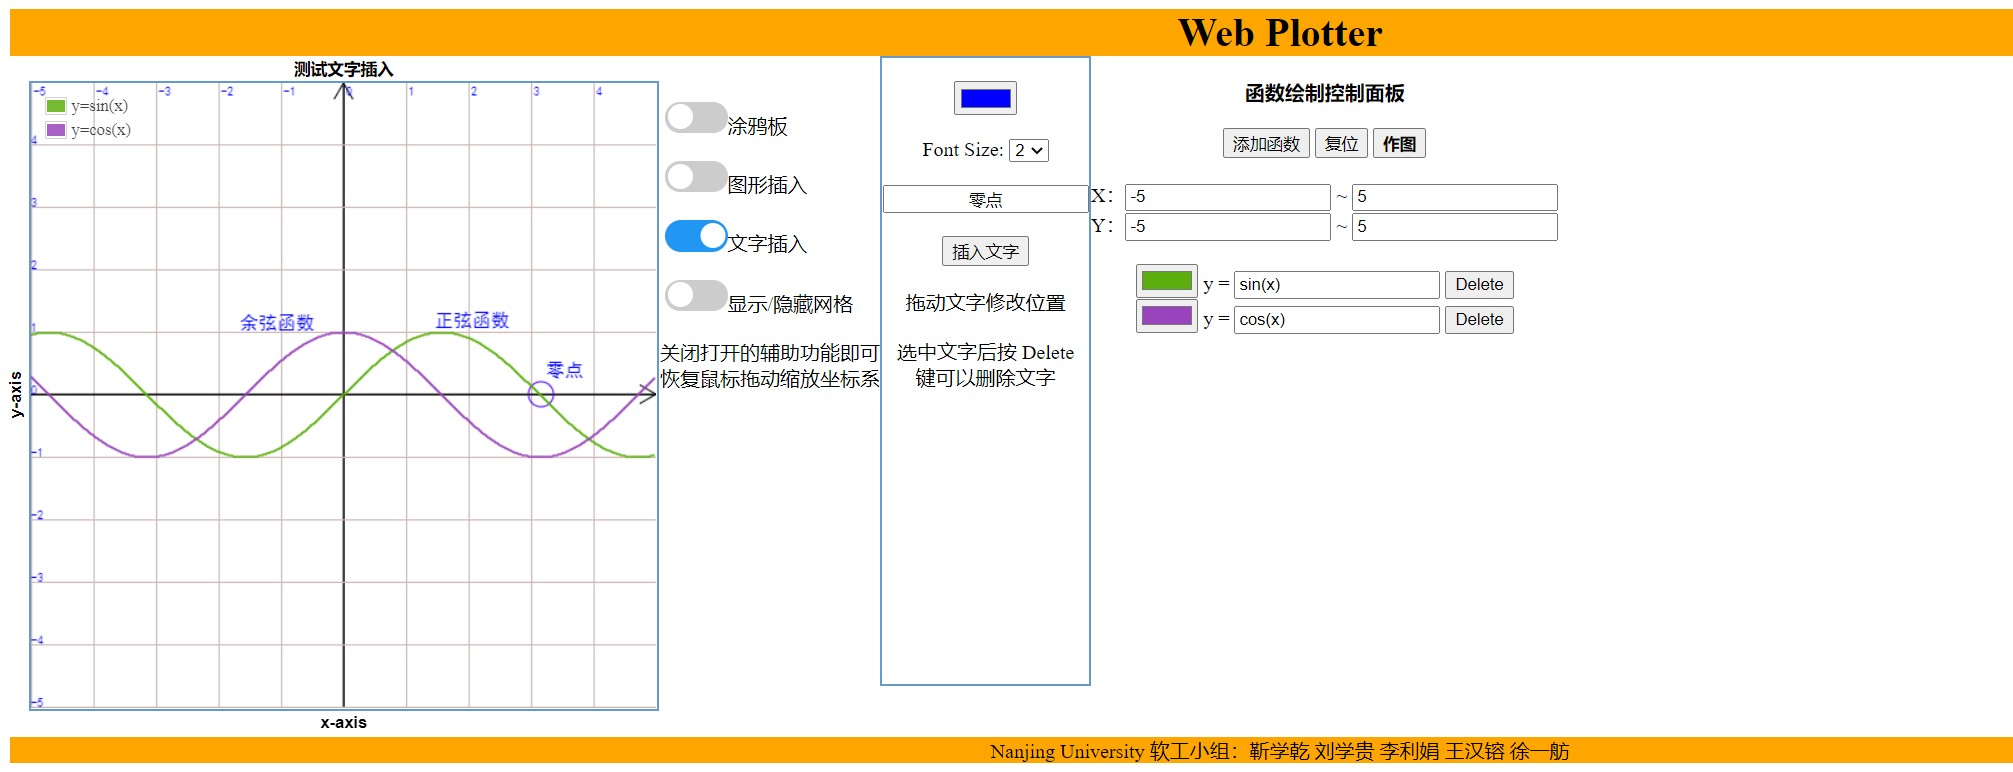
\includegraphics[width=1.0\textwidth]{5.jpg}
	\caption{测试文字插入效果}
	\label{5img}
\end{figure}

\subsection{测试总结}

在测试过程中发现了一些潜在的错误,将这些错误改正后,网页作图系统能正常运行,满足工程文档中的需求,性能满足预期要求。

要站在用户角度对系统进行测试。从一些项目中出现的未能及时发现的bug中,要认识到用户体验的重要性。

与开发人员的沟通很重要。测试过程中不管遇到什么不确定或疑惑,都要及时与开发人员沟通,提高工作效率。

\section{项目总结}
本次软件工程大作业,我们完整地经历了一次软件开发的流程,体会到了一个团队应该如何配合工作才会更加高效,避免陷入1+1<2的局面。总体上有以下几点感悟:
\begin{itemize}
	\item [(1)]加强团队交流:团队内部成员定期进行交流十分重要,我们组每周召开一次例会,在做项目过程中如果有成员有问题直接将问题发到讨论群里,大家一起商量解决,如果线上说不清楚,积极线下商讨。项目组内的各成员及时将自己的想法和意见表达出来,更好的协同工作,可以提高项目组的开发效率。
	\item [(2)]制定阶段性目标:制定阶段性的小目标具有重要意义,每周制定每周任务,并及时完成,项目前期,我们组内大部分成员的阶段性目标都不是特别明确,开发效率较低,好在我们及时发现和解决这个问题,开始制定周目标、日目标,项目组整体的开发效率得到了大大的提升。
	\item [(3)]进行前期分析设计:前期的分析与设计工作是整个项目的基础,前期分析不清晰,后期的工作量将会倍增,本次项目开发过程中,在前期对整个系统模块进行设计时,有一处的细节处理并不是特别的完善,导致后期各端在实现相应需求时工作量倍增。
	\item [(4)]掌握甲方需求:上课听老师讲课特别重要,老师相当于我们的甲方,我们要准确了解甲方的需求才能使做出来的产品得到认可,同时老师也会给指导性的意见,避免我们做很多不必要的工作。
	\item [(5)]代码模块化:在合适的情况下,可以适当增强模块代码的独立性,提高相似功能的开发效率,同时也可以减小后期修改的工作压力。一开始我们在开发过程中,部分几个小功能模块功能相似,未及时抽象出来,导致后续工作进展不顺,后面重构部分代码,解决了这一问题。
	\item [(5)]注重测试过程:之前上课听老师讲测试部分内容可能多少有点不以为意,觉得代码写出来,可以运行应该就没有什么问题。但这次的经历让我们深刻体会到测试在软件开发过程的重要性,通过测试,我们发现一些从代码层面看不出来的问题,并最终完善相应功能。
\end{itemize} 

总之,在这次网页作图实践中,我们小组成员收获颇多。从设计到实现网页作图,各种功能都需要我们自己想办法实现。刚开始我们感觉很难入手,但是不管遇到多少困难也坚持到最后。通过查阅书籍、上网搜索资料以及小组成员之间的交流,我们最终还是较好地完成了作图网页。

在整个过程中,我们收获了许多知识,尤其是对于网页编程的理解更加深刻,有些知识书本上面看到的和实践中获得的是不一样的,也正印证了那句话:纸上得来终觉浅,绝知此事要躬行。软件工程不仅仅需要理论知识,更要有实践能力的配合和支撑。此外,小组成员之间的合作较好地锻炼了大家的团队合作能力,为我们今后参与大型软件项目的开发打下了良好基础。
















% include the noncited reference
% \nocite{ref1, ref2}
% \bibliographystyle{aer}
% \bibliography{wpref}
\end{document}
\end{lstlisting}

\nocite{*}

% 如果想修改参考文献样式(非国标),请把下行取消注释,并换成合适的样式(比如 unsrt,plain 样式)。
%\bibliographystyle{aer}
\bibliography{wpref}

\end{document}
